\documentclass{article}

% Macros to make this problem look like the rest of our problems.
\usepackage{icpc_problem}
\usepackage{graphicx}

% Title of your problem.
\title{J: Knight's Tour}

% Who made the problem
\author{Charles Riedesel}

% Keywords, from a set of standard keywords.
\keywords{simple}

% Anything you want to say about the problem, including how one could solve it
\comments{Picture a simple polygon on a checkerboard grid.  How many moves are
needed for a knight to visit each square in the grid at least once. Solution:
Simple BFS, watching for shortest paths as vertices are visited from other
branches.}

% Difficulty on a 1..10 scale.
\difficulty{1}

\begin{document}

\begin{problemDescription}
Knights on a chessboard have very interesting ways to move.  They jump (ignoring
the contents of squares being jumped) from one square to a new square that is at
the opposite corner of a 2 by 3 grid of squares stretching in any direction.
Studying their possible movements is a popular passtime of puzzle solvers.  This
exercise solves one of these puzzles.

Imagine a grid bounded by a simple rectilinear polygon.  In this polygon is placed
a knight.  The knight needs to reach a princess who is also in the polygon.  It is
essential to reach the princess in the fewest possible jumps.  Each jump must keep
the knight in the polygon, though he may jump over intervening edges if there is
some contiguous path in the polygon on the 2 by 3 grid that defines the jump 
(as described above).  Your task is to help the knight by telling him what the 
minimum number of jumps is.  While it would be polite to report the details of 
the path, that is beyond the scope of your responsibility.

\vspace{-0.7in}
\begin{center}
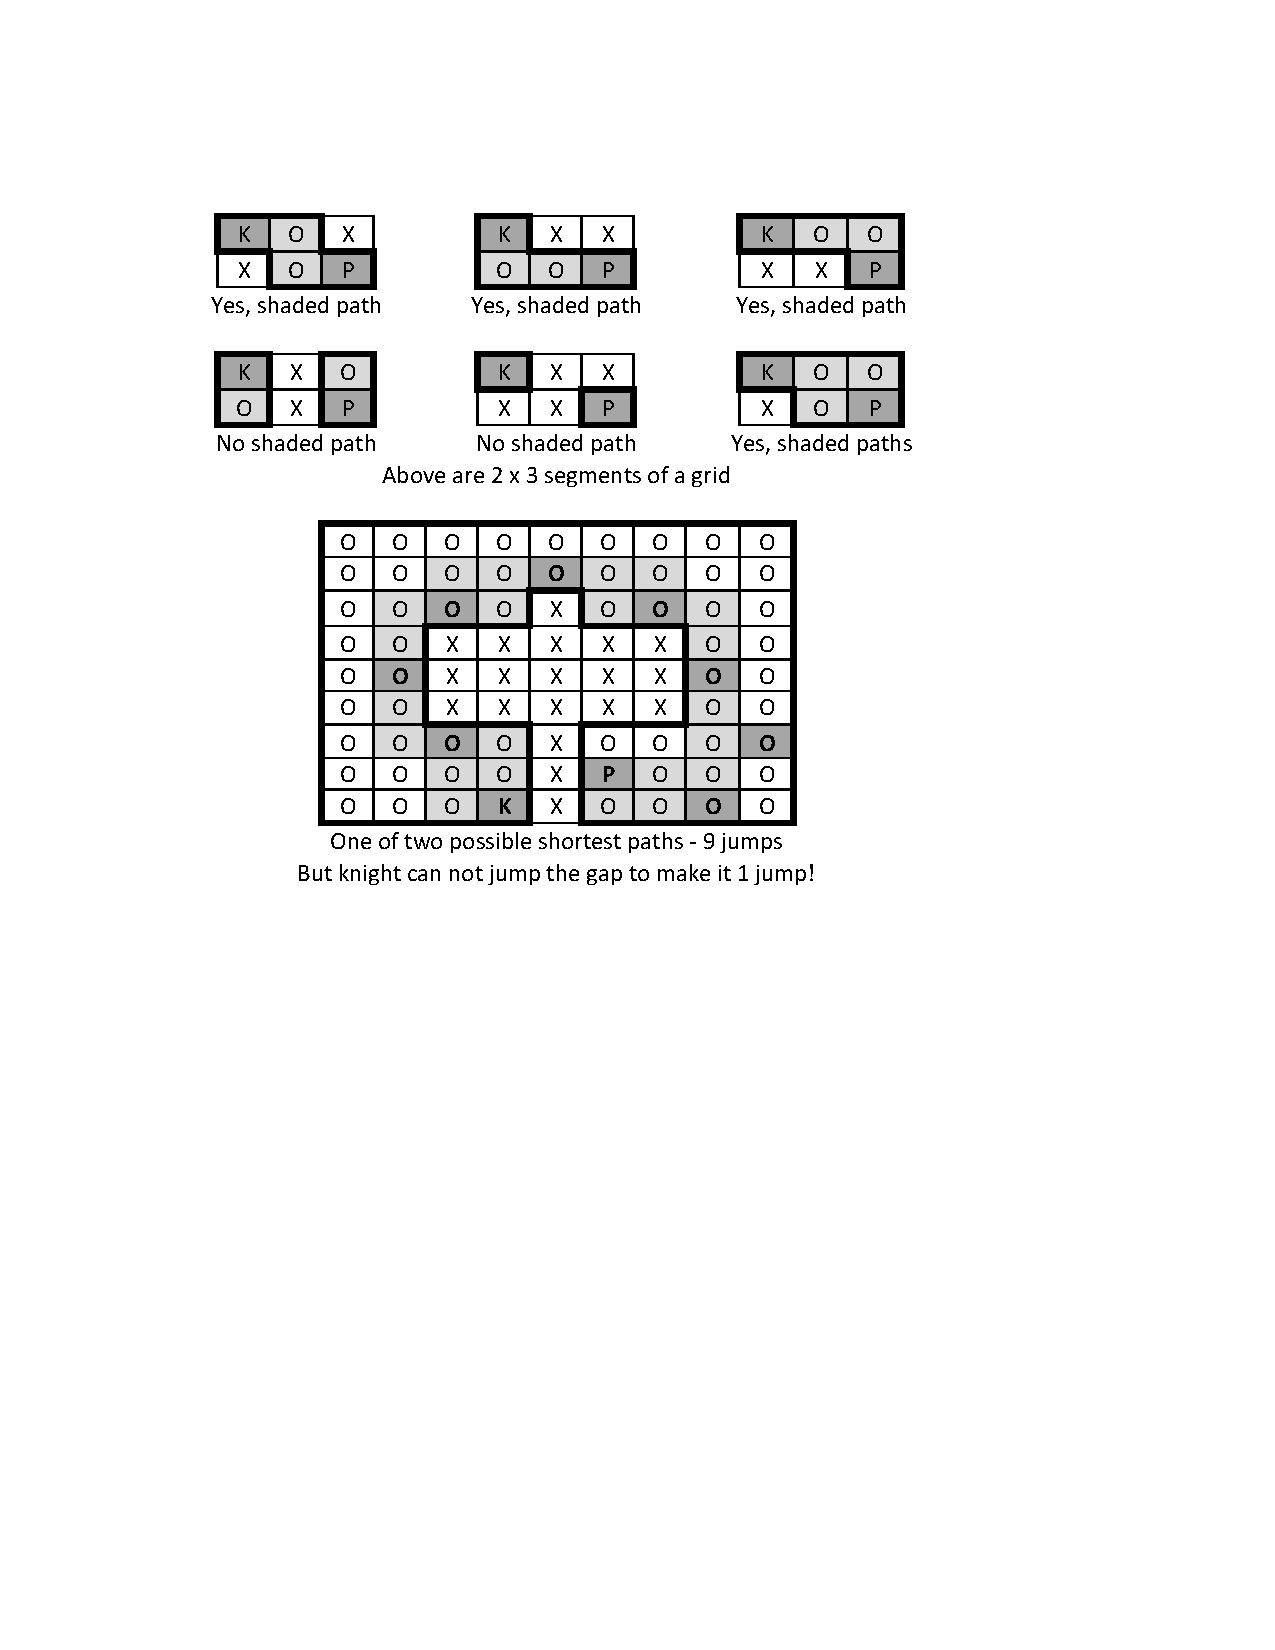
\includegraphics[scale=0.55]{knightstourFigure.pdf}
\end{center}
\vspace{-2.0in}

\end{problemDescription}

\begin{inputDescription}
Input may consist of multiple cases.  Each case begins with a line containing
the number of rows and columns of the playing board.  Neither of these will 
be more than 100.  The details of the board are 
shown in the next lines, one line per row.  The row is represented as a string
whose characters indicate if the corresponding grid positions are outside the
bounding polygon $(X)$, inside the bounding polygon $(O)$, the position of the
knight $(K)$, and the position of the princess $(P)$.  The knight and princess will
both be inside the bounding polygon.  The last case is followed by a line 
containing two 0's.  Arbitrary white space may be used as delimiters.
\end{inputDescription}

\begin{outputDescription}
For each case, display the case number followed by the fewest possible jumps,
formatted as in the sample.  If it is not possible to reach the princess, say
``impossible" as shown below.  Use single spaces as delimiters.
\end{outputDescription}

\begin{sampleInput}
1    6
  XKOOPX
2 5
KOXOP
XOOOX
2 5
KOXOP
XXOOX
0 0
\end{sampleInput}
\begin{sampleOutput}
Case 1: impossible
Case 2: 2
Case 3: impossible
\end{sampleOutput}

\end{document}
